\chapter{RCNSP的设计与实现}
本章介绍规则自动补全的神经符号VQA框架(Rule Complement Neuro-Symbolic Pipeline, RCNSP),
下面分别从RCNSP设计方案、RCNSP核心技术及实现、实验分析三个方面进行详细阐述。
\section{RCNSP设计方案}
RCNSP框架的架构设计方案如图\ref{fig:pipeline}所示。框架的整体设计思路是:
在框架初始化阶段,规则蒸馏模块依据LLM中蕴含的大量知识生成ASP规则,进而获得较为完整的ASP知识库。
在框架运行阶段,视觉场景理解模块从输入的图像中抽取
物体所在区域、物体属性等信息,并以ASP形式进行表示;另一方面,语义解析模块对输入的自然语言问题进行解析,
同样以ASP形式进行表示,并由迭代反馈与规则修正模块对生成的ASP规则进行修正。
随后将ASP知识库、图像、问题三个方面的ASP规则统一输入ASP推理模块进行求解。如果对某个问题无法求解出正确答案,
规则蒸馏模块会尝试进行生成新规则,实现ASP知识库的动态更新。
最后,由于ASP推理模块输出的是ASP语句,
可读性较差,普通用户难以理解,因此需要求解结果翻译模块将其翻译为自然语言形式进行输出。
\begin{figure}[h]
    \centering
    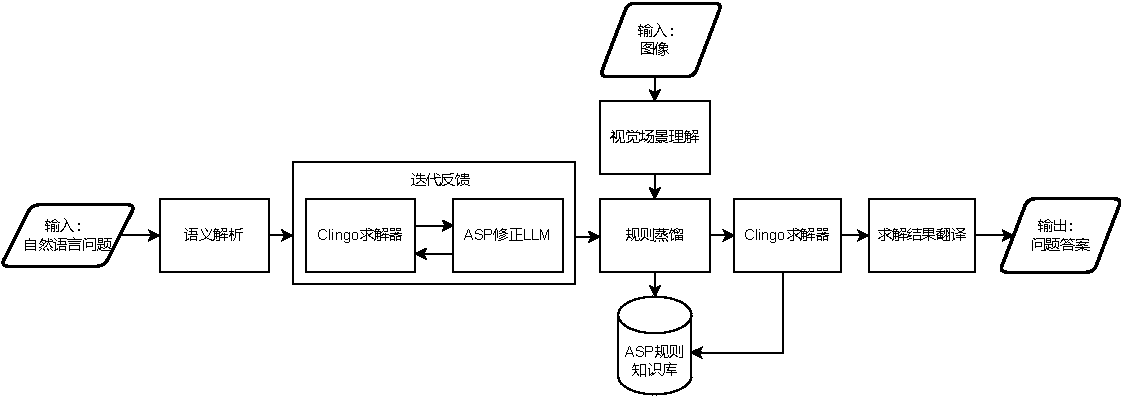
\includegraphics[width=\textwidth]{figures/pipeline-crop.pdf}
    \caption{面向空间推理领域的神经符号框架示意图}
    \label{fig:pipeline}
\end{figure}
\subsection{视觉场景理解}
本模块的任务是从输入的积木世界图像中检测积木物体并提取其属性(颜色、形状、大小、材质)、位置以及相互之间的空间关系,并把
这些视觉信息转换为符号化的ASP事实(如\texttt{color(obj1,red)}、\texttt{shape(obj1, cube)}、\texttt{left(obj1,obj2)}等)。
具体可采用YOLO、GLIP等目标检测技术识别所有物体并分类其属性,然后通过深度估计或多视角几何计算获得物体在空间中的坐标。
检测结果生成ASP事实,作为后续推理的输入。本模块也是经典的神经符号VQA流水线中,使用深度学习技术进行感知的关键一环。

面临的挑战主要有:积木世界场景物体外观简单而同质化,易混淆且纹理缺乏区分度,加之物体之间经常出现遮挡(尤其是立体堆叠时),导致信息不完整。
遮挡使得部分物体属性或空间信息丢失,需要推理补全。此外,物体的精确位置和深度估计存在误差可能引发推理偏差。
如何在低分辨率或部分可见条件下准确提取场景结构,是视觉理解模块的关键挑战。

技术方法上,
\subsection{语义解析}
语义解析模块的目标是将用户的自然语言问题转化为可在积木世界中执行的ASP查询,以支持后续推理。
例如,将问题“Which red object is on the top of the blue cube?”转化为ASP的形式。

研究中面临的难题在于,自然语言的歧义性和多样性使得准确解析为ASP规则具有挑战性,例如“besides”可能有多种解释。
另外,积木世界中的对象属性(颜色、形状)和空间关系(上、下、左、右)需要精确的符号表示,而这些信息可能因表述不同而难以统一。

技术方法上,本模块针对积木世界中常见的属性查询问题进行了优化,
例如通过训练模型识别“next to”、“besides”、“nearby”等词,并将其映射到明确的ASP谓词。创新点在于,本文在此提出了一种数据增强策略,利用
积木世界场景生成的合成问答对来微调模型,从而提升其在特定领域的解析能力。
这种方法特别适用于处理积木世界中独特的语言模式,例如与空间推理相关的复杂问题。

相较于通用的语义解析方法,本模块的方法更专注于积木世界中的结构化语言特性,能够更高效地处理涉及物体属性和空间关系的问题,
减少歧义解析的错误率。
\subsection{迭代反馈与规则修正}
本模块的任务是在通过语义解析模块得到ASP查询之后,进行多轮迭代检查与修正,确保ASP查询正确无误,可以顺利通过Clingo执行。

本模块研究中的难点在于,LLM在生成ASP规则时容易出错,且目前学术界和工业界很少有关于ASP规则修正的微调数据集,难以采用
微调的方法对生成ASP规则进行优化。

技术方法上,本文设计了多种提示模板,通过DSPy框架对LLM进行提示词优化,使模型在无需重新训练的情况下,自动学习如何更有效地修正 ASP 程序,
同时提示词优化降低了对大量高质量标注数据的需求,很大程度上解决了本模块研究中的难题。

本方法相比已有工作的创新点在于,已有工作中的ASP代码修正依赖于预先定义的ASP错误类型和修正策略。而本方法通过引入Clingo的执行反馈提示,
指导提示词的动态变化,在保持模型参数不变的前提下,显著提高了ASP程序的可执行性和准确率。
\subsection{规则蒸馏}
本模块旨在从LLMs中提取简洁且准确的ASP规则,用于积木世界的推理任务。
具体应用主要包括两方面:一是在RCNSP初始化阶段,利用“LLMs基于海量语料预训练,包含
丰富的知识”这一特性,将LLMs中蕴含的知识转换为可执行、可解释的ASP规则的,用于完善初始ASP知识库。
二是在RCNSP运行阶段,当出现对某个问题无法求解出正确答案的情况时,
规则蒸馏模块会尝试进行生成新规则,实现ASP知识库的动态更新。

本模块研究的难点在于,在RCNSP初始化阶段对积木世界VQA数据集进行蒸馏的过程中,当样本的数量过多时,进行全量蒸馏
可能会耗时过长,同时也能会引入一些对解决积木世界VQA问题无关的冗余知识。这些冗余知识在每次ASP推理时,都要输入到Clingo中,
当RCNSP处理用户VQA请求数量逐步增加时,因冗余知识而导致的累计性能损耗也将逐步增大。

技术方法上,本模块通过构建初始ASP知识库,并以本文构建的积木世界数据集POVQA\-D为样本进行蒸馏,生成积木世界空间推理所需的ASP规则并完善ASP知识库。
另外在RCNSP运行过程中,当出现知识不足,无法求解的情况时,规则蒸馏模块将会引导LLM生成新的ASP规则以补充ASP知识库。
同时,本模块在蒸馏过程中采用了样例选择策略,减少无关数据的干扰,避免全量蒸馏,实现了蒸馏性能优化,解决了本模块研究中的难点。

与已有工作中传统的模型压缩式蒸馏不同,本方法强调将LLM中“隐式的知识”显式地提取为ASP规则。
而规则蒸馏的本质是将大语言模型中蕴含的知识,转换为可执行、可解释的逻辑规则,用于扩展已有的推理系统。
\begin{enumerate}[nosep]
\item \textbf{启发式拓展}:以经迭代反馈修正后得到的ASP规则和视觉场景理解模块生成的ASP规则为基础,当发现这些ASP规则无法解答某个问题时,引导LLM生成新的规则。
\item \textbf{以数据为指导而非训练为导向}:不训练模型,而是以示例为提示,向LLM提出规则生成任务。
\end{enumerate}
\subsection{ASP推理}

\subsection{求解结果翻译}

在框架的整个工作流水线中,始终以ASP作为知识表示形式和贯穿整个框架的核心。对输入的自然语言问题
和图像,都需要对其进行转换,将其中的信息以ASP的形式进行表示,以便后续ASP求解器进行推理。因此,
需要视觉场景理解模块将图像中的信息提取出来,并以ASP的形式进行表示;同时,也需要语义解析模块
将自然语言问题解析成ASP规则。

经语义解析模块解析后的ASP规则,可能会存在一些错误,例如语法错误等等。为了保证ASP程序能够正常运行,
故在语义解析模块之后,增加了一个迭代反馈与规则修正模块。该模块的主要作用是对解析后的ASP规则进行修正,
因为可能存在单次修正不能发现全部错误,或者单次修正之后又产生新的错误的情况,故采取多次迭代的方式进行修正,
直到可以通过Clingo运行或者达到最大次数(默认3次)为止。由于LLM在自然语言处理方面的强大能力,以及
部分研究表明LLM在代码生成方面取得了显著的成功\cite{gao2023pal,he2023solving},故在迭代反馈与规则修正模块中,
引入LLM对ASP程序进行修正。

本文研究的是部分可见积木世界场景下的空间推理问题,在部分可见场景中,模型可能无法从图像中获取所有的知识,
需要利用一些已有常识作为补充。而Wang\cite{wang2024dspy}等人提出的神经符号框架中,并未支持自动化拓展
ASP规则。为了减轻开发人员的负担,本文添加了规则蒸馏模块。该模块的主要作用是对迭代反馈修正后的ASP规则进行补全,
以便满足问题对相关背景知识的需求。

经过Clingo得到的输出结果,以形式化的ASP谓词表示,难以直接为最终用户所理解,对用户而言并不友好,需要将其转为自然语言。
而LLM在自然语言处理方面的强大能力,可以将ASP规则翻译为自然语言形式,便于用户理解。故在最后设置了一个求解结果翻译模块,
负责将Clingo的输出ASP语句翻译为自然语言形式。

LLM在整个框架中的作用有以下四点:
\begin{enumerate}[nosep]
    \item 在语义解析模块中,LLM对自然语言问题进行语义解析,将问题以ASP的形式表示出来,以便后续
输入到迭代反馈模块中进行修正。
    \item 在迭代反馈模块中,LLM对ASP表示进行多次迭代优化,其中包括解析错误、基础化错误等。每一轮迭代都将
根据上一轮的错误信息进行针对性的修正。
    \item 在规则蒸馏中,LLM结合ASP知识库中的先验知识,对迭代反馈修正后ASP规则进行进一步补全,为Clingo求解器
推理提供更全面的知识。
    \item 在求解结果翻译中,LLM 将 Clingo 求解器输出的 ASP 表达结果翻译为自然语言形式,以回答提出的问题。
\end{enumerate}
\section{RCNSP核心技术及实现}
\subsection{视觉场景理解}
视觉场景理解的目标是从输入图像中提取结构化信息,包括物体的属性(如形状、颜色、大小等)、位置信息以及物体间的空间关系。
这些信息将被进一步转换为ASP的形式,为后续基于逻辑推理的语义解析与问答模块提供形式化的知识基础。

本节主要围绕以下四个方面展开详细阐述:目标检测、空间位置提取、空间关系提取以及场景生成。
最后,给出一个完整的视觉场景理解演示案例,并讨论在实现过程中遇到的关键技术挑战及相应解决方案。
\subsubsection{目标检测}
目标检测是视觉场景理解的最基本的任务,其目标是从图像中识别出所有相关物体,并标注其边界框、类别和属性。本文选择GLIP模型作为目标检测的实现工具,原因在于
其独特的语言-视觉预训练特性。基于大规模的图文对数据,GLIP进行大量预训练,能够根据自然语言描述(如“红色立方体”)直接定位图像中的对应物体。
这种能力特别适合VQA任务,使问题中的语言信息与图像内容高效对齐成为可能。

目标检测是视觉场景理解的基础任务,其任务是从输入图像中识别出所有相关物体,
并为每个物体确定其边界框、类别和相关属性。本文采用了GLIP模型作为目标检测的核心工具,其主要优势体现在:
\begin{enumerate}[nosep] 
\item \textbf{语言-视觉预训练能力:}GLIP在大规模图文对数据上进行预训练,能够根据自然语言描述(例如“红色立方体”)直接定位图像中的对应物体,从而实现图像内容与问题描述的高效对齐; 
\item \textbf{高效性与鲁棒性:}模型在处理多样化场景时具有较高的检测准确率,适合构造后续依赖视觉信息的场景图。 
\end{enumerate}

具体实现流程如下:
\begin{enumerate}[nosep] 
\item \textbf{图像预处理:}将原始图像调整至GLIP模型要求的输入分辨率(例如800$\times$1333像素),
以保证检测精度; 
\item \textbf{文本提示构造:}根据数据集构造要求,设计一组覆盖目标类别及属性的自然语言提示。
本文选取的提示短语包括描述物体大小(如“大物体”、“小物体”)以及颜色与形状组合(如“红色立方体”、“蓝色球体”、“绿色圆柱体”等); 
\item \textbf{目标检测与属性解析:}将图像和文本提示输入GLIP,获得每个检测物体的边界框和类别标签。随后对类别标签进行解析,将复合描述(如“红色立方体”)拆解为单独属性(color=red, shape=cube)。同时,通过计算边界框面积($(x_2 - x_1)\times(y_2 - y_1)$),结合预设阈值进一步推断物体的大小属性。 
\end{enumerate}

例如,对于一张包含“红色立方体”和“蓝色球体”的图像,GLIP可能检测出如下信息: 
\begin{enumerate}[nosep] 
\item 物体1:类别为“红色立方体”,边界框坐标为$(x_1, y_1, x_2, y_2)$; 
\item 物体2:类别为“蓝色球体”,边界框坐标为$(x_3, y_3, x_4, y_4)$。 
\end{enumerate}
\subsubsection{空间位置提取}
在完成目标检测后,接下来的任务是为每个物体确定其精确的空间位置,这对于后续空间关系的推理至关重要。
本文采用以下两种方式提取物体位置信息:
\begin{enumerate}
\item \textbf{二维中心点计算}:利用目标检测得到的边界框信息,计算物体在图像平面内的中心点坐标。公式如下:
$$x_c = \frac{x_1+x_2}{2}, y_c = \frac{y_1 + y_2}{2}$$
该中心点坐标用于描述物体在二维图像中的位置;
\item \textbf{三维位置信息获取}:若图像同时包含深度信息(例如通过Blender渲染生成的场景),则可直接从深度图中提取物体的z值,从而获得物体在三维空间中的位置,
表示为$(x, y, z)$。
\end{enumerate}

提取出的位置信息将以ASP事实的形式进行存储,例如:position(obj1, x1c, y1c, z1) 表示物体1的中心点位置。
\subsubsection{空间关系提取}
空间关系的提取是实现复杂场景理解与多步逻辑推理的关键。本文从以下几个角度对空间关系进行提取:
\begin{enumerate}[itemsep=0.5em] 
\item \textbf{二维空间关系:}基于物体的中心点坐标计算物体之间的相对位置。例如: 
    \begin{itemize}[leftmargin=2em] 
        \item 若物体A的$x_c$小于物体B的$x_c$,则判定A位于B的左侧,表示为\texttt{left(objA, objB)}; 
        \item 类似地,通过比较$y_c$坐标可判定上下关系(例如,若物体A的$y_c$小于B,则A在B之上,记作\texttt{above(objA, objB)})。 
    \end{itemize} 
\item \textbf{三维空间关系:}利用深度信息,对物体间的前后关系进行判断。
例如,若物体A的z值小于物体B的z值,则判定A位于B的前面,记作\texttt{in\_front\_of(objA, objB)}。 
\item \textbf{遮挡关系:}结合边界框重叠情况与深度信息进行判断。如果两个物体边界框存在重叠且A的深度值明显小于B,
则可以认为A遮挡B,记作\texttt{occludes(objA, objB)}。 
\end{enumerate}
所有提取到的空间关系均转换为ASP事实,如:
left(obj1, obj2) 表示物体1在物体2的左边,in\_front\_of(obj1, obj2) 表示物体1在物体2的前面;
occludes(obj1, obj2) 表示物体1遮挡了物体2。
\subsubsection{场景图生成}
场景图是将目标检测、空间位置与空间关系综合融合成的统一结构化表示,其主要构成如下: 
\begin{enumerate}[nosep] 
    \item \textbf{节点表示:}每个节点对应图像中的一个物体,并附有相应的属性(如color, shape, size, material)以及位置信息; 
    \item \textbf{边的构建:}节点之间的边用于表示物体间的空间关系,如left\_of、in\_front\_of等。 
\end{enumerate}

在构建过程中,首先为每个检测到的物体创建一个节点,并记录其属性及位置;
随后,依据前述空间关系,将相应的有向边添加到图中。
最终,整个场景图将被转化为ASP事实,以支持后续符号推理任务。
\subsubsection{实现细节与实例}
为便于说明,下面给出一个具体示例。假设输入图像包含如下场景: 
\begin{enumerate}[nosep] 
    \item 一个红色大立方体位于图像左侧; 
    \item 一个蓝色小球体位于图像右侧,且位于红色立方体的前方。 
\end{enumerate}

经过GLIP目标检测,得到如下检测结果: 
\begin{itemize}[itemsep=0pt,parsep=0pt] 
    \item 物体1:类别为“红色立方体”,边界框为(50, 100, 150, 200); 
    \item 物体2:类别为“蓝色球体”,边界框为(250, 50, 350, 150)。 
\end{itemize}

进一步计算得到: 
\begin{itemize}[itemsep=0pt,parsep=0pt] 
    \item 物体1的中心点坐标为$(100,150)$; 
    \item 物体2的中心点坐标为$(300,100)$。 
\end{itemize}

假设深度信息显示:物体1的z值为50,物体2的z值为75,则可提取以下空间关系: 
\begin{itemize}[itemsep=0pt,parsep=0pt] 
    \item \texttt{left\_of(obj1, obj2)}(因为100 $<$ 300); 
    \item \texttt{above(obj2, obj1)}(因为100 $<$ 150); 
    \item \texttt{in\_front\_of(obj2, obj1)}(因为75 $>$ 50,在三维空间中深度值较大的物体更靠后,需根据具体定义调整)。 
\end{itemize}

最终生成的ASP事实示例如下: 
\begin{lstlisting}[language=Prolog] 
color(obj1, red). 
shape(obj1, cube). 
size(obj1, large). 
position(obj1, 100, 150, 50).

color(obj2, blue). 
shape(obj2, sphere). 
size(obj2, small). 
position(obj2, 300, 100, 75).

left_of(obj1, obj2). 
above(obj2, obj1). 
in_front_of(obj2, obj1). 
\end{lstlisting}
\subsubsection{技术挑战与解决方案}
在实际实现过程中,本模块面临如下关键技术挑战,并提出相应解决方案: 
\begin{enumerate}[nosep] 
    \item \textbf{检测准确性}:GLIP 在处理物体密集或遮挡严重的场景时,可能存在误检问题。为此,本文引入非极大值抑制(NMS)以及深度信息辅助过滤,提高检测精度; 
    \item \textbf{空间关系鲁棒性}:二维关系受视角影响较大,为增强鲁棒性,本文在有深度信息的条件下优先采用三维关系,并结合几何约束(例如边界框重叠)进行补充; 
    \item \textbf{计算效率}:面对大规模图像数据,为保证系统实时性,本文通过批量处理图像以及优化提示设计,有效降低了GLIP的推理延时。
\end{enumerate}
\subsubsection{小结}
本节详细介绍了基于GLIP的视觉场景理解模块的整体架构与实现细节。
通过对目标检测、空间位置与空间关系的综合提取,最终构建了能够转化为ASP事实的场景图,
为后续语义解析和逻辑推理提供了坚实的数据基础。
下一节将介绍如何利用LLM将自然语言问题转化为ASP查询,实现语义解析与神经符号推理的无缝衔接。
\subsection{语义解析}
语义解析的主要任务是使用 LLM 将自然语言问题转换为 ASP 表达形式,获得ASP规则,以便后续与视觉场景理解提取的场景事实结合进行逻辑推理。

直观上,LLM可能很难直接解决复杂的推理问题。然而,LLM已经在理解文本输入并将其转化为形式化程序方面取得了巨大成功,
例如程序代码\cite{gao2023pal}和数学方程\cite{he2023solving}。为了让LLM更准确地生成ASP编码,本文在此对通用LLM进行针对性微调。
\subsubsection{微调数据集模板设计}
现有的通用代码生成数据集可能无法充分覆盖ASP中普遍存在的特定结构和模式,而对LLM针对特定任务进行微调,面向特定领域的数据集必不可少。
因此,对LLM针对ASP编码任务进行微调的核心是:创建一个涵盖多种ASP问题类别的微调数据集。
通过创建一个有针对性的数据集,模型可以更有效地学习这些特定的细微差别。

本文以下对常见的ASP编程任务进行分析,确定了以下9种ASP编码的基本情形,分别为其设计模板,用于后续构建微调数据集。
\begin{enumerate}[nosep]
\item \textbf{猜测赋值}是ASP编码中的经典情形。具体而言,猜测赋值指的是将某一给定集合中的所有元素赋予一个从固定集合中选出的唯一标签。
在ASP中,通常使用析取来表示“猜测”。以下是猜测赋值的一个示例。
\begin{lstlisting}
模板:为以下问题编写一个 ASP 程序。在给定的一组标签中,为元素集准确分配一个标签。元素集由谓词 [PREDICATE] 表示。标签为 [LABEL]+。
提示:为以下问题编写一个 ASP 程序。在给定的一组标签中,为元素集准确分配一个标签。元素集由谓词 city 表示。标签为 moscow、rome、dubai。
编码:assign(X,"moscow") |assign(X,"rome") | assign(X,"dubai") :- city(X).
\end{lstlisting}
\item \textbf{表达约束}表示必须满足的条件。在ASP中,这通常通过(经典/强)约束来实现,有时会使用辅助规则。以下是表达约束的一个示例。
\begin{lstlisting}
模板:为以下问题编写一个 ASP 程序。防止值为 [VALUE] 的谓词 [PREDICATE] 带有标签 [LABEL]。
提示:为以下问题编写一个 ASP 程序。防止值为 11 的谓词 car 带有标签“red”。
编码: :- assign(11,"red").
\end{lstlisting}
\item \textbf{生成组合}指创建来自两个不同集合的所有可能的元素组合(笛卡尔积)。在ASP中,可以通过简单的规则完成。以下是生成组合的一个示例。
\begin{lstlisting}
模板:为以下问题编写一个 ASP 程序。从两个集合生成所有元素组合。这两个集合分别由谓词 [PREDICATE_1] 和 [PREDICATE_2] 表示。
提示:为以下问题编写一个 ASP 程序。从两个集合生成所有元素组合。这两个集合分别由谓词 city 和 airport 表示。
编码: combination(X,Y) :- city(X), airport(Y).
\end{lstlisting}
\item \textbf{连接}指的是基于特定匹配标准将来自两个不同集合的元素关联起来。在ASP中,通常通过在规则体中具有共享变量的文字来定义。以下是连接的一个示例。
\begin{lstlisting}
模板:为以下问题编写一个 ASP 程序。假设谓词 [PREDICATE_1] 具有字段 [LABEL]+,谓词 [PREDICATE_2] 具有字段 [LABEL]+。定义一个谓词 [PREDICATE_1]_[PREDICATE_2],将每个 [PREDICATE_1] 与 [PREDICATE_2] 的 [LABEL] 关联。
提示:为以下问题编写一个 ASP 程序。假设谓词“owner”具有字段“ID”、“surname”、“name”、“restaurantID”,谓词“restaurant”具有字段“ID”、“description”。定义一个谓词“owner_restaurant”,将每个所有者与餐厅的描述关联。
编码:owner_restaurant(X,Z) :-owner(X,_,_,Y),restaurant(Y,Z).
\end{lstlisting}
\item \textbf{传递闭包}用于定义超出直接连接的关系,捕获由一系列关系形成的间接关系。在ASP中,通常需要多个规则,通常涉及递归。以下是传递闭包的一个示例。
在该示例中,编码使用了两条规则:一条用于定义直接关系,另一条(依赖递归)用于捕捉间接关系。
\begin{lstlisting}
模板:为以下问题编写一个 ASP 程序。将谓词 [PREDICATE_1] 定义为谓词 [PREDICATE_2] 的传递闭包。
提示:为以下问题编写一个 ASP 程序。将谓词“arrivals”定义为谓词“flight”的传递闭包。
编码:arrivals(X,Y) :- flight(X,Y).
arrivals(X,Y) :- flight(X,Z),arrivals(Z,Y).
\end{lstlisting}
\item \textbf{表达偏好}用于定义对一组可接受解决方案的偏好,通常用于解决优化问题。在ASP中,通常通过编码带有弱约束的程序来完成。以下是表达偏好的一个示例。
\begin{lstlisting}
模板:为以下问题编写一个 ASP 程序。我希望值为 18 的谓词 [PREDICATE] 与 [LABEL] 不相关联。如果发生这种情况,则在级别 [LEVEL] 上花费 [COST]。
提示:为以下问题编写一个 ASP 程序。我希望值为 18 的谓词 house 与“flat”不相关联。如果发生这种情况,则在级别 2 上花费 2。
编码::∼assign(18,"flat").
\end{lstlisting}
\item \textbf{按值过滤}的过滤标准是:选取某个谓词外延中与特定值匹配的部分。
以下是按值过滤的一个示例。
\begin{lstlisting}
模板:为以下问题编写一个 ASP 程序。选择与标签为 [LABEL] 的谓词 [PREDICATE] 相关联的所有值。
提示:为以下问题编写一个 ASP 程序。选择与标签为“purple”的谓词 color 相关联的所有值。
编码:select(X) :- color(X,"purple").
\end{lstlisting}
\item \textbf{负过滤}的过滤标准是:排除与给定条件匹配的谓词扩展部分。具体而言,可以是两个谓词外延之间的差集(减法运算),也可以是复合条件的否定。
以下是负过滤的一个示例。
\begin{lstlisting}
模板:为以下问题编写一个 ASP 程序。选择与谓词 [PREDICATE_1] 关联但与谓词 [PREDICATE_2] 和标签 [LABEL] 不关联的所有值。
提示:为以下问题编写一个 ASP 程序。选择与谓词 vehicle 关联但与谓词 moto 和标签“kawasaki”不关联的所有值。
编码:select(X) :- vehicle(X),
not moto(X,"kawasaki")。
\end{lstlisting}
\item \textbf{按数值比较过滤}的过滤标准是:根据项之间比较的结果,对表格中部分内容进行过滤。
以下是按数值比较过滤的一个示例。
\begin{lstlisting}
模板:为以下问题编写一个 ASP 程序。选择与谓词 [PREDICATE] 关联且值大于或等于 [VALUE] 的所有值。
提示:为以下问题编写一个 ASP 程序。选择与谓词 size 关联且值大于或等于 5 的所有值。
编码:select(X) :- size(X,C), C>=5。
\end{lstlisting}
\end{enumerate}

通过明确定义不同ASP任务的模板,可以系统地生成数据,确保覆盖基本的ASP概念,并允许在需要时系统地扩展数据集。
使用模板可以程序化地生成庞大且多样化的数据集,这比手动创建大型数据集更有效且更可控。

\subsubsection{微调数据集生成}
本文将所需生成的微调数据集记为$D$,包含自然语言描述的ASP任务及其对应的标准ASP程序片段,二者构成一个二元组。
数据集的结构基于一个模板集$T = (P, A)$,其中$P$是自然语言描述的集合,$A$是ASP程序的集合 。
T进一步划分为${TC_1, TC_2,..., TC_k}$,每个$TC_i$代表一种特定的任务类型,例如猜测赋值、表达约束、生成组合、连接、传递闭包、表达偏好和过滤。

对于每种任务类型,通过实例化包含谓词、标签和值的占位符来生成模板的变体,这些谓词、标签和值来自预定义的集合 。由此产生的完整数据集$D$大约包含3.7万个元组 。
数据集中不同任务类型元组的数量占比取决于每种任务所需的ASP代码的句法复杂性,具体各类型占比见表\ref{tab:task-portion}。
对应ASP程序中变异性较大的任务(例如规则中谓词数量、原子元的元数(arity)、以及实例的具体化情况)在训练过程中需要更多数据。
最终,数据集被分成训练集(80\%)和验证集(20\%),并且在两个集合中都保持了每种问题类型的比例 。

\begin{table}[ht]
\centering
\begin{tabular}{lrr}
\toprule
\textbf{ASP任务类型} & \textbf{元组数量} & \textbf{占比(\%)} \\
\midrule
赋值          & 10000 & 27.0 \\
约束          &   5000 & 13.5 \\
组合         &   1000 & 2.7 \\
连接                &   9000 & 24.3 \\
闭包  &   1000 & 2.7 \\
偏好          &   4000 & 10.8 \\
按值过滤     &   1000 & 2.7 \\
负过滤  &   1000 & 2.7 \\
按数值比较过滤   &   5000 & 13.5 \\
\midrule
\textbf{Total}      & 37000 & 100 \\
\bottomrule
\end{tabular}
\caption{微调数据集中的各类型ASP任务数量及其占比}
\label{tab:task-portion}
\end{table}

\subsubsection{模型选择与微调}
目前,工业界已推出众多LLM,这些LLM在架构、参数量和训练数据集等方面各有不同。本文聚焦于一些开源LLM,这些开源的LLM也代表了当前LLM领域的最新研究成果。
选用的LLM如下:
\begin{enumerate}[nosep]
\item \textbf{ChatGPT-4o}:由OpenAI于2024年发布的多语言、多模态LLM。
\item \textbf{DeepSeek-Coder}:由深度求索公司发布的开源代码大模型系列,专注于代码生成、补全、调试及跨语言转换等编程任务。
\item \textbf{LLaMA3}:LLaMA 模型的增强版,在推理、代码生成和遵循指令等任务中有显著提升。
\end{enumerate}
表\ref{tab:llm-comparison}简要对比了所选LLM的参数规模、架构和训练数据来源。
从中可以识别出两个模型规模群体:一个是大型模型组(参数量 ≥ 700 亿),另一个是小型模型组(参数量 < 700 亿);其中DeepSeek-Coder 1.3B是本次实验中体积最小的模型。

\begin{table}[ht]
    \centering
    \begin{tabular}{lccc}
        \toprule
        \textbf{模型} & \textbf{参数量} & \textbf{架构} & \textbf{训练数据源} \\
        \midrule
        ChatGPT-4o    & 200B      & 多模态统一网络           & 网络数据         \\
        DeepSeek-Coder       & 1.3B--33B      & MoE + MLA            & 网络数据    \\
        LLaMA3         & 8B--70B   & 纯解码器 + 分组查询注意力机制   & 网络数据         \\
        \bottomrule
    \end{tabular}
    \caption{LLM对比详细信息}
    \label{tab:llm-comparison}
\end{table}

在众多模型中,本文选用DeepSeek-Coder 1.3B作为微调模型。选择其的主要原因是,其体积是当前主流可用模型中最小的,
在其上进行微调能够充分验证即便是在小规模的LLM上,本文的微调也能够显著提升性能。
训练方法上采用了标准的监督式微调(Supervised Fine-Tuning, SFT),
同时为了节省内存和计算资源,使用了QLoRA技术。
训练工具采用了trl库中的SFTTrainer。硬件环境上,CPU为Intel Core i9 12900K,内存为128GB,显卡为2张Nvidia RTX4090。
微调数据集选用上一小节中构造的微调数据集的训练集部分(占总数据集的80\%)。

\subsubsection{评估指标}
评估指标选用语法准确率和语义准确率,使用ASP求解器Clingo执行ASP程序,进而判断语法、语义是否正确。对于一个程序$P$,Clingo用于计算该程序的答案集。
进而该过程可以等价于:定义一个函数$f(P) = AS(P)$,其中$AS(P)$表示程序P的所有回答集(可能为空)。

LLM根据提示$x$生成的ASP程序,记为$y ~ P_L(|x)$。与$x$对应的能够真实表示问题的标准ASP程序,记为$y^*$。按照以下步骤来进行验证:
首先基于$x$构建一个表示具体实例的事实集$F_{y^*}$。接着,构造两个完整的ASP程序:
\begin{enumerate}[nosep]
\item $P = y \cup F_{y^*}$:由模型生成程序与事实集合成的程序。
\item $P^* = y^* \cup F_{y^*}$:由标准程序与事实集合成的程序。
\end{enumerate}

此后,执行以下评估步骤:
\begin{enumerate}
\item 语法检查:调用Clingo运行程序$P$,若未发生解析错误,则认为模型生成的程序 $y$ 在语法上是正确的,则判定为语法命中。否则,则判定为不命中。
\item 语义检查:分别用 Clingo 计算$f(P)$与$f(P^*)$,分别得到各自的答案集$AS(P)$与$AS(P^*)$。若$AS(P)$与$AS(P^*)$完全匹配,则判定为语义命中。
否则,则判定为不命中。
\end{enumerate}
\subsection{迭代反馈与规则修正}
迭代反馈模块是整个VQA框架的核心部分,
其主要功能在于对语义解析模块生成的ASP程序进行检查,如果有错误,则使用LLM对其进行修正。
\subsubsection{流程概述}
整个迭代反馈与规则修正的大致流程如下:
\begin{enumerate}[nosep]
\item 使用Clingo求解器对语义解析模块生成的ASP程序尝试执行。
\item 如果执行成功,没有提示错误,则无需进行进一步修正,直接将ASP程序流转到框架的下一模块。
\item 如果执行失败,则将错误的ASP程序和Clingo求解器提示的错误信息,一起输入LLM,由LLM尝试进行修正。
\item 将修正后的ASP程序再次输入到Clingo求解器中,尝试执行。如此循环最多3次,最终输出经过优化后的ASP程序,流转到框架的下一模块。
\end{enumerate}
\subsubsection{错误类型与修正策略}
不同类型的错误信息对应着ASP程序中不同的问题,因此需要采用不同的修正策略。本文设计了多套提示模板,用以指导LLM针对性地进行程序修正。
\begin{enumerate}[nosep]
\item \textbf{语法错误}:这类错误通常发生在程序违反了ASP的语法规则时。错误信息会指出文件、行号、列号以及意料之外的符号 。例如,遗漏句点、括号不匹配或使用了Clingo版本不支持的语法都可能导致语法错误 。
以下是该错误的一个提示词模板:
\begin{lstlisting}
任务描述:请根据提供的 ASP 程序和 Clingo 错误信息,对程序进行修正。

错误类型:语法错误 (Syntax Error) - 规则或事实缺少句号。

错误程序:
node(a).
node(b) % <- 错误:这里缺少句号
edge(a, b).

path(X, Y) :- edge(X, Y).
path(X, Z) :- edge(X, Y), path(Y, Z).

Clingo错误信息:
<stdin>:3:1: error: syntax error, unexpected IDENTIFIER, expecting '.' or ':
  node(b) % <- 错误:这里缺少句号

修正后程序:
node(a).
node(b). % <- 修正:添加句号
edge(a, b).

path(X, Y) :- edge(X, Y).
path(X, Z) :- edge(X, Y), path(Y, Z).
\end{lstlisting}
\item \textbf{谓词未定义}:这通常是一个警告,表示某个谓词在规则体中被使用,但从未在任何规则的头部定义过 。
程序执行不会因此停止,但可能暗示着逻辑错误 。以下是该错误的一个提示词模板:
\begin{lstlisting}
任务描述:请根据提供的 ASP 程序和 Clingo 错误信息,对程序进行修正。

错误类型:未定义的谓词(Undefined Predicate)

错误程序:
p(a) :- q(a).

Clingo错误信息:
error: in rule at line 1: undefined predicate: q/1

修正后程序:
q(a).
p(a) :- q(a).
\end{lstlisting}
\item \textbf{循环负依赖}:循环负依赖发生在程序的依赖图中存在负循环,即一个谓词通过一系列规则负依赖于自身。
负循环可能导致程序没有解答集。​此外在某些情况下,可能导致多个解答集的产生,增加了解释的复杂性。以下是该错误的一个提示词模板:
\begin{lstlisting}
任务描述:请根据提供的 ASP 程序和 Clingo 错误信息,对程序进行修正。

错误类型:​递归中的负循环(Negative Cycle in Recursion)​

错误程序:
p(X) :- not q(X).
q(X) :- not p(X).

Clingo错误信息:
error: in rule at line 2: cyclic dependency: p/1 -> q/1 -> p/1

修正后程序:
p(X) :- r(X), not q(X).
q(X) :- s(X), not p(X).
\end{lstlisting}
\item \textbf{重复的规则或者事实}:这类错误往往是由于人为输入错误或多个ASP程序进行合并时,没有去重导致。以下是该错误的一个提示词模板:
\begin{lstlisting}
任务描述:请根据提供的 ASP 程序和 Clingo 错误信息,对程序进行修正。

错误类型:​重复的规则或事实(Duplicate Rules or Facts)​

错误程序:
p(a).
p(a).

Clingo错误信息:
warning: fact at line 2 is a duplicate of fact at line 1

修正后程序:
p(a).
\end{lstlisting}
\item \textbf{约束条件恒为假}:在ASP中,约束条件的作用是排除使Body为真的解答集。
当约束条件的Body部分恒为真时,该约束条件始终排除所有可能的解答集。出现这一错误时,由于所有可能的解答集都被排除,程序将没有解答集,即程序不一致。
\begin{lstlisting}
任务描述:请根据提供的 ASP 程序和 Clingo 错误信息,对程序进行修正。

错误类型:​约束条件总为假(Constraint Always False)

错误程序:
:- p(X), not p(X).

Clingo错误信息:
warning: constraint at line 1 is always false

修正后程序:
:- p(X), not q(X).
\end{lstlisting}
\item \textbf{不安全变量}:当一个变量出现在规则的头部,但没有在规则体的任何肯定字面量中出现时,就会发生这种错误 。这可能会导致产生无限的稳定模型 。Clingo会报告出错的规则以及不安全的变量名 。以下是该错误的一个提示词模板:
\begin{lstlisting}
任务描述:请根据提供的 ASP 程序和 Clingo 错误信息,对程序进行修正。

错误类型:基础化错误 (Grounding Error) - 规则中存在不安全变量。

错误程序:
reachable(X) :- edge(Y, X). % <- 错误:变量 Y 是不安全的,因为它没有在规则头或任何正文字面量中安全出现

Clingo错误信息:
<stdin>:5:20-21: error: variable Y is unsafe
  reachable(X) :- edge(Y, X). % <- 错误:变量 Y 是不安全的...

修正后程序:
reachable(X) :- edge(Y, X), node(Y). % <- 修正:添加 node(Y) 来约束 Y 的范围
\end{lstlisting}
\item \textbf{不一致的事实和规则}:如果程序中定义的事实和规则之间存在矛盾,会导致出现逻辑错误。以下是该错误的一个提示词模板:
\begin{lstlisting}
任务描述:请根据提供的 ASP 程序和 Clingo 错误信息,对程序进行修正。

错误类型:逻辑错误 (Logical Error) - 程序包含直接冲突的规则或事实,导致没有稳定模型。

错误程序:
light_on. % 灯是开着的

:- light_on. % 约束:灯不能是开着的

Clingo 错误信息:
Reading from <stdin>
Solving...
UNSATISFIABLE

Models       : 0
Calls        : 1
Time         : 0.000s (Solving: 0.00s 1st Model: 0.00s Unsat: 0.00s)
CPU Time     : 0.000s

修正后程序 (根据意图选择修正): (修正方法取决于真实意图。这里假设约束是错误的)
light_on. % 灯是开着的

% :- light_on. % <- 修正:注释掉或删除冲突的约束
(或者,如果事实是错误的)
% light_on. % <- 修正:注释掉或删除冲突的事实

:- light_on. % 约束:灯不能是开着的
\end{lstlisting}
\end{enumerate}
每一轮反馈过程中,LLM都将结合Clingo返回的错误信息和预定义的提示模板进行针对性修正,
从而使生成的ASP程序在下一轮执行中更趋于正确和可执行。

\subsubsection{提示词优化}
本小节中采用DSPy框架对LLM进行提示词优化,以提升模型在ASP规则修正中的准确性和可执行性。不同于传统的微调方法,
本节未直接修改LLM的内部权重参数,而是通过优化模块化提示词,使模型在无需重新训练的情况下,自动学习如何更有效地修正ASP程序。

如果直接使用LLM进行ASP规则修正,容易出现以下问题:
\begin{enumerate}[nosep]
\item 生成的ASP规则存在语法错误或逻辑错误;
\item 不同LLM(如GPT-4 mini、Llama3等)间推理风格差异大,直接迁移困难。
\end{enumerate}

传统的全量微调在一定程度上可以缓解上述问题,但目前学术界和工业界很少有关于ASP规则修正的微调数据集,而且
微调往往需要大量高质量标注数据。因此,本文选择通过提示词优化,以更低的代价提升模型在ASP修正任务中的推理能力,同时保持系统的灵活性与可解释性。

本节基于DSPy进行提示词优化,具体过程如下:
\begin{enumerate}[nosep]
\item \textbf{模块定义}:将ASP程序修正任务进行拆解,形成标准化模块。每个模块中需要定义输入和输出
\item \textbf{训练数据准备}:本文使用上一节人工设计的错误修正提示模板作为小规模训练样本,每个样本包括错误的ASP程序、错误类型、正确的ASP程序。例如:
\begin{lstlisting}
from dspy import example

examples = [
    Example(
        inputs={
            "error_code": "node(a). node(b) edge(a,b). path(X,Y) :- edge(X,Y). path(X,Z) :- edge(X,Y), path(Y,Z).",
            "error_description": "Missing period at the end of rule.",
            "error_type": "<stdin>:3:1: error: syntax error, unexpected IDENTIFIER, expecting '.' or ':node(b)"
        },
        outputs={
            "corrected_code": "node(a). node(b) edge(a,b). path(X,Y) :- edge(X,Y). path(X,Z) :- edge(X,Y), path(Y,Z)."
        }
    ),
    ...
]
\end{lstlisting}
使用少量高质量示例,能够有效指导LLM理解常见的ASP错误模式,并通过优化提示方式学会修正,而无需大规模标注数据,显著降低数据需求。
\item \textbf{提示词优化}:对模块进行提示学习。
在提示词优化过程中,DSPy会动态尝试不同提示策略(如补充细节描述、修改模板结构等),修改
提示词中问题引导方式、任务定义、输出格式要求等内容,并且比较各提示版本的准确率,选择最佳版本。
由于LLM的推理质量极大程度上受提示词的影响,通过系统化地优化提示,而不是依赖手工试错,可以稳定、高效地提升推理准确性,
同时避免人为偏差。
\end{enumerate}
\subsection{规则蒸馏}
\subsubsection{设计思路}
规则蒸馏的流程如图\ref{distill-process}所示。首先,构建一个初始的ASP知识库,包含一些手动编写的、部分完备的规则集合。
此后,本文采用POVQAD数据集中的训练集,对ASP知识库进行补充,形成初步完善的ASP知识库。在RCNSP执行用户命令时,
规则蒸馏模块会检查是否当前ASP规则是否完善,如果有补充的需要,则会基于ASP知识库执行运行时规则拓展。补充完成之后,
继续进行RCNSP的其它环节。
\begin{figure}[h]
    \centering
    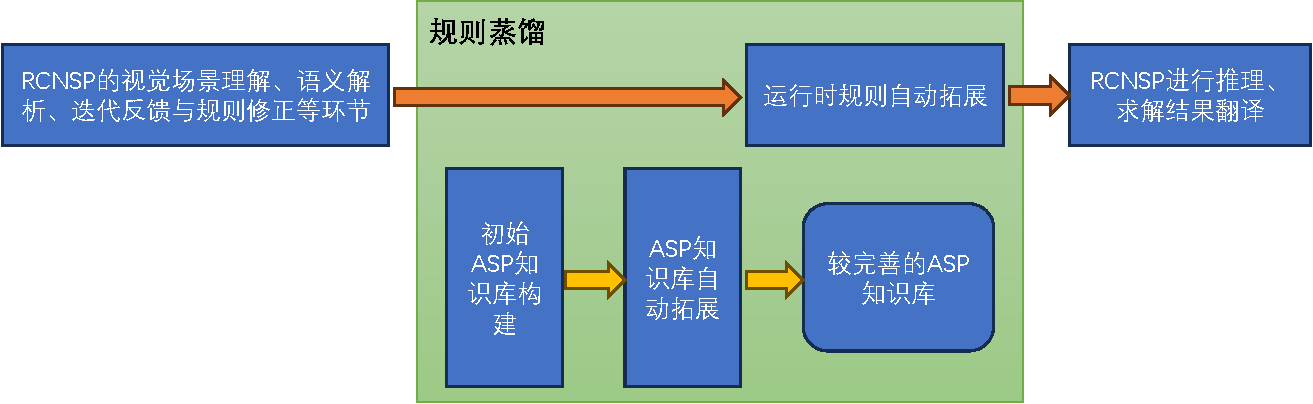
\includegraphics[scale=0.7]{figures/distillation-crop.pdf}
    \caption{规则蒸馏流程图}
    \label{distill-process}
\end{figure}
\subsubsection{初始ASP知识库构建}
初始ASP知识库是整个规则蒸馏方法的起点,其中包含了一些人工编写的、部分完备的规则集合,用于支持VQA系统在一定程度上进行逻辑推理。
执行VQA任务的过程中,问题的多样性和复杂性导致很难一次性将所有知识都填充到ASP知识库中。
因此,需要构建一个初始ASP知识库,后续再不断对其拓展和完善。

初始ASP知识库的构建遵循“最小可运行”的原则,即在保证系统能够正确回答部分问题实例的前提下,
仅包含最基本的一些ASP规则。
这样做一方面保证了系统可以运行并进行基本验证,另一方面也为LLM提供了清晰、结构化的理论框架,
使其可以基于已有规则进行合理补全。

初始ASP知识库中通常包含以下几个方面的规则:
\begin{enumerate}[nosep]
\item 基本推理操作规则,包括属性过滤(如\texttt{filter\_color}、\texttt{filter\_shape})、
对象选择(\texttt{select})、合取与析取(\texttt{and}、\texttt{or})、数量计算(\texttt{count})、
布尔值判断(\texttt{exist}、\texttt{verify\_attr}、\texttt{verify\_rel})等等。例如:
\begin{lstlisting}
state(TO,ID) :- scene(TO), object(ID).  % 初始状态:每个object都在scene中
state(TO,ID) :- select(TO, TI, CLASS), state(TI, ID), has_attr(ID, class, CLASS).
bool(TO,yes) :- or(TO, TI0, TI1), bool(TI0,yes).
ans(V) :- end(TO), attr(TO,V).
:- not ans(_).  % 强制必须产生答案
\end{lstlisting}
以上这些规则都使用变量表达,而非常量,以保持泛化能力。
\item 根据数据集中常见问题需求构建规则。POVQAD中,问题均围绕物体的属性、物体的区域位置进行提问。
可以根据数据集中的问题类型,构建一些常见的规则,例如针对提问目标物体的颜色的问题,可能要用到物体的
其它属性、所在的区域等信息来间接推理,可以构建\texttt{filter\_shape}、\texttt{fiter\_region}、
\texttt{filter\_material}、\texttt{filter\_size}规则,
其作用是根据物体的形状、区域、材质、大小等属性进行过滤,从而帮助找出目标物体。
\end{enumerate}

在初始ASP知识库构建过程中,当系统识别到当前知识库无法覆盖某个问题时(例如ASP求解器无法推出目标答案、
产生错误答案或触发语法异常),便会将场景的ASP表示、问题的ASP表示与答案一起作为输入提示给LLM,
要求其生成扩展规则用于补全初始ASP知识库。新生成的规则在通过语法检查和规则一致性检查后,将被追加至初始ASP知识库中,
以支持对更广泛问题的解答。语法检查通过Clingo对新生成规则试运行来实现,若没有错误,则认为语法正确;
规则一致性检查通过将新生成规则与现有规则进行合并,
然后用Clingo进行求解,若没有出现错误,表明没有出现ASP规则互相矛盾的情况,则认为规则一致性检查通过。

通过这种基于“最小起点+增量学习”的构建思路,实现了初始ASP知识库向任务完备理论的动态演进,
兼顾了系统可解释性、扩展性与开发效率。
\subsubsection{ASP知识库自动拓展}
在初始ASP知识库构建完成后,本文采用了基于LLM驱动的规则自动拓展机制,以实现对ASP知识库的自动拓展。
数据集选用POVQAD数据集中的训练集,使用其中每个样本数据中的问题的ASP表示$QA_i$、场景$S_i$和答案集$A_i$,
同时将初始ASP知识库记作$K$。将$QA_i$、$S_i$和$K$共同输入Clingo,查看是否能够得到答案$A_i$。
如果能够得到答案$A_i$,则说明当前的ASP知识库包含了足够解决该问题的知识,无需将该问题及其答案用于ASP知识库拓展。
如果不能得到答案$A_i$或者出现了语法错误的情况,则需要使用LLM生成规则,对当前的ASP知识库进行拓展。

ASP知识库的自动拓展包括以下几个步骤:预提示、规则生成、规则验证。

预提示的作用是,为 LLM 提供背景信息和任务说明。具体而言,预提示包括以下内容:
\begin{enumerate}[nosep]
\item \textbf{任务介绍}:首先简要说明 VQA 任务的背景,告诉 LLM 任务的性质——给定一个问题、
一个图像和它们的描述,生成相应的答案。
\item \textbf{语言语法}:介绍 ASP 规则的基本语法和约定。具体而言,ASP 使用了一些类似于逻辑
程序设计的语法,如:-(表示规则的条件)和 not(表示否定)。
\item \textbf{场景与问题解释}:解释如何将图像场景和问题转换成 ASP 的表示方式。
\item \textbf{答案格式}:告诉LLM如何表示和返回问题的答案。
\item \textbf{初始ASP知识库}:提供初始的ASP知识库$K$,能够回答部分问题,但可能做不到回答所有问题。
\end{enumerate}

该机制通过增量式规则扩展实现 ASP 知识库的动态演进:每当系统识别出现有理论无法
推导正确结果时,会触发 LLM 的规则生成模块,输出符合 ASP 语法的逻辑规则补充到 ASP
知识库中。整个过程形成“问题识别-规则生成-理论扩展”的闭环优化路径。

以下为节选的部分提示词,可作为参考:
\begin{lstlisting}
你的任务是对ASP知识库进行维护,通过动态更新规则确保其能够解答各类问题。ASP知识库中的现有规则已能够满足对部分问题的处理需要,需根据输入的问题的ASP表示进行增量式规则拓展。输入提示将包含一个或多个采用ASP表示形式的问题。请严格遵守以下规则:

1. 仅输出新增的ASP规则。
2. 禁止将事实作为规则添加。不允许在规则头(head)中使用具体常量实例。
3. 将规则的泛化程度实现最大化。你输出的规则应具备以下特征:使用大写字母变量(如X,Y,Z)替代具体常量,通过谓词逻辑建立抽象关系而非具体实例关联。
4. 完全禁用自然语言。你的输出中,不得出现任何自然语言成分,包括:错误提示信息、代码注释说和解释性文字。
\end{lstlisting}

在向 LLM 进行预提示之后,将问题的ASP表示$QA_i$、场景$S_i$一同作为附加提示,要求LLM生成新的ASP规则。
生成的规则是尽可能一般化的规则,即包含更多的变量和较少的常量,以便可以适用于
更广泛的情况。例如,如果问题是“这只杯子是什么颜色?”,LLM 可能会生成以下 ASP 规则:
\begin{lstlisting}
color_of_cup(Color) :- object(Cup), has_attr(Cup, color, Color), class(Cup,cup).
\end{lstlisting}
这条规则表示:“如果某个物体是杯子,并且它有颜色属性,那么可以推理出它的颜色”。

规则生成之后,需要验证生成的规则是否正确。这一过程需要进行语法
检查、语义检查和回归测试。

语法检查的目的是:检查生成的规则是否符合 ASP 的语法要求。如果规则存在语法错误,
例如拼写错误或格式不对,ASP 解析器将无法解析这些规则。在这种情况下,系统会将错误
信息反馈给 LLM,并要求 LLM 进行迭代反馈修正。

语义检查的目的是:检查生成的规则是否能够配合原有规则,获得预期的答案$A_i$。如果
不能通过语义检查,则采取“反馈+重试”的方法试图进行修正:将Clingo输出的答案与期望的标准答案一同作为追加提示
提供给LLM,并且新的提示词中会明确告知LLM“你之前生成的规则未能得到正确答案,请你根据下面的输入修改规则。”,
LLM会基于原问题、场景、当前规则结果与目标答案的对比,尝试修复逻辑错误或补全缺失的中间推理步骤。
对同一个示例最多允许修正尝试的次数设为m,其默认值为1,表示失败一次就修正一次,防止过多LLM调用。
若修正后仍失败,说明当前LLM无法处理该示例,跳过或保留当前状态。

语法检查和语义检查都是涉及LLM对ASP程序进行修正,故采用迭代反馈与规则修正中经过训练的LLM来完成此处的
语法检查和语义检查任务。

回归测试的目的是:在扩展 ASP 理论的同时,确保新规则不会导致旧问题的答案错误。这
一设计主要基于以下几方面的考量:
\begin{enumerate}[nosep]
\item \textbf{维护系统稳定性和一致性}: 在软件工程中,回归测试被广泛应用于验证新代码的引入
是否影响现有功能的正确性。类似地,在 VQA 系统中,每当通过知识蒸馏添加新规则
时,需要确保这些规则不会干扰系统对先前问题的解答。
\item \textbf{应对模型更新带来的潜在风险}: 知识蒸馏的过程涉及从教师模型向学生模型传递知识,
可能导致学生模型的行为发生变化。通过回归测试,可以检测并防止新知识引入后对模
型性能的负面影响。
\item \textbf{借鉴软件开发中的最佳实践}: 在软件开发中,回归测试是确保新功能或修改不会引入
新错误的关键步骤。将这一理念应用于 VQA 系统,有助于在不断扩展和优化系统的同
时,保持其可靠性和准确性。
\end{enumerate}

回归测试的具体步骤如下:基于更新后的 ASP 理论,重新执行所有历史测试用例,确保
所有旧问题仍然能得到正确答案。如果某个旧问题的答案被破坏,则回退到先前的 ASP 理论,
并要求 LLM 重新修正生成的规则。
通过上述设计,回归测试在ASP知识库自动拓展过程中起到了关键的质量保证作用,确
保系统在不断学习和扩展的同时,保持其稳定性和可靠性。

语法检查、语义检查和回归测试这三个环节中,任意一处的修正经多次尝试失败后,系统将视为该问题暂时无法解决,会进行跳过处理。
\subsubsection{蒸馏性能优化}
POVQAD训练集中包含数万个样例,如果直接对样本进行蒸馏,既耗时又可能引入冗余信息。
因此,为了提高蒸馏效率,本文提出了样例选择策略,以减少无关数据的干扰。具体而言,包
括以下两种方法:
\begin{enumerate}[nosep]
\item \textbf{谓词计数策略}:该策略根据 ASP 问题表示中谓词的数量对实例进行分组。 分组方法是:
统计每个问题表示中出现的谓词数量,并将具有相同谓词数量的问题归为一组。 通过
这种分组方式,可以根据问题的复杂度(即涉及的谓词数量)来选择示例。 这有助于
LLM 在训练过程中逐步学习,从处理简单问题(谓词数量少)开始,逐步过渡到复杂问
题(谓词数量多),从而提高生成规则的准确性和泛化能力。
\item \textbf{谓词相关性策略}:该策略根据 ASP 问题表示中涉及的具体谓词对实例进行分组。分组
方法是: 识别每个问题表示中出现的谓词,并将包含相同谓词的问题归为一组。 通过
这种分组方式,可以确保 LLM 针对特定谓词学习相关规则。 这有助于 LLM 深入理解
每个谓词的作用和使用场景,从而生成更精确的 ASP 规则,提升 VQA 系统在处理涉及
特定谓词的问题时的表现。
\end{enumerate}

谓词计数策略的设计借鉴了课程学习的思想。课程学习是一种训
练策略,强调按照从易到难的顺序逐步引入训练样本,以提高模型的学习效果。谓词计数策
略通过问题复杂度的分层,体现了课程学习的理念,使模型能够在逐步增加的复杂度中稳定
学习。

在自然语言处理和知识表示领域,基于谓词的特征选择方法被广泛应用于文本分类和信
息检索等任务。谓词相关性策略吸取了这一方法的经验,通过关注问题中涉及的具体谓词,利
用领域知识进行特征选择,确保模型关注于最相关的信息,提高推理的准确性。

为了进一步提高效率,本文还提出了批量优化策略,即一次性给 LLM 多个示例,而不是
逐个示例地生成规则。这一策略借鉴自 Ge\cite{ge2021selfdistillationbatchknowledgeensembling} 等人提出的批量知识集成的自蒸馏方法。 在知
识蒸馏领域,批量知识集成方法通过在同一小批量内传播和整合样本间的知识,生成更精确
的软目标,从而提升模型性能。此外,自蒸馏方法利用模型自身的预测作为训练目标,减少
对外部教师模型的依赖,简化训练流程。

采用批量优化策略,具有以下几点突出优势:
\begin{enumerate}[nosep]
\item \textbf{提高训练效率}: 通过在同一批次内处理多个样本,模型可以并行学习不同样本的特征
和模式,减少训练时间。
\item \textbf{增强模型泛化能力}:批量优化允许模型在一个批次内接触多样化的数据,帮助模型学习
更广泛的特征表示,从而提升对未见数据的适应能力。
\item \textbf{优化资源利用}:通过批量处理,能够更有效地利用计算资源,减少训练过程中的开销。
\end{enumerate}

综合来看,批量优化策略通过借鉴批量知识集成和自蒸馏等方法,旨在提升知识蒸馏过
程中的训练效率和模型性能。
\subsubsection{运行时规则自动拓展}
ASP知识库经过自动拓展之后,包含了一定量的知识,能够处理一些POVQAD中的一些问题。
用户将自然语言问题和对应积木世界图像输入RCNSP,经过语义解析、视觉场景理解、迭代反馈与规则修正后,
由规则蒸馏模块进行处理。与框架初始化阶段进行ASP知识库构建时的规则蒸馏不同,运行时规则自动拓展的目的是:
利用ASP知识库中已有的知识,对用户输入的问题、图像所对应的ASP规则进行补充,以解决部分可见积木世界场景中的
空间推理问题。

判断是否需要进行规则自动拓展的依据是:将问题的ASP表示$QA_i$与场景的ASP表示$S_i$共同输入Clingo,查看是否能够得到答案。若出现语法错误或者无解,则表明
当前ASP规则不足,需要进一步补充。若能够输出与问题相关的ASP谓词(如,问题提问的是不可见物体的颜色,输出谓词也是与颜色相关),则表明
已经有足够的解决问题的规则,不需要进一步补充,直接将$QA_i$和$S_i$继续向后传递到ASP求解器中进行正式求解即可。

此处拓展规则的设计思路与ASP知识库自动拓展中的思路基本相同,不同的点在于,此处输入的只有问题的ASP表示$QA_i$、
场景的ASP表示$S_i$,而不包括问题的答案。由于输入LLM的提示发生了变化,因而提示词也有所变化。
最终接收的输出是新生成的ASP规则。在生成过程中,同样也进行规则验证,并采用反馈重试的方法试图进行修正。
\subsection{ASP推理}
ASP推理阶段中,ASP求解器接收经过优化后的ASP查询语句、视觉场景理解模块提取的ASP事实以及自动拓展的ASP规则,
进行逻辑推理,最终获得答案。
本文使用Clingo求解器来进行求解,其工作过程分为基础化(grounding)阶段和求解(solving)阶段。

基础化阶段将ASP程序中的变量替换为常量,生成一个新的ASP程序。Clingo
通过使用内置的基础化器分析程序,生成所有可能的规则。例如,对规则
$a(X) :- b(X), not c(X).$,其将被展开为所有可能的值为X的实例。

求解阶段中,Clingo采用类似SAT求解器的冲突驱动答案集求解(CDNL)方法。CDNL方法通过迭代地添加约束,
直到找到一个满足所有约束的解,或者证明无解。
具体而言,Clingo基于如下步骤进行求解:(1)初始化。从空分配开始(没有原子被标记为真);
(2)选择与分配。选择一个未分配的原子,猜测其真值为真或假;
(3)传播。根据当前分配和规则,推导其他原子的真值。例如,若规则$a :- b, not c.$满足,b为真且c不在答案集中,则a必须为真;
(4)冲突检测。若分配导致规则冲突(如与已有的约束条件相抵触),记录冲突原因;
(5)回溯与学习。若发生冲突,回溯到之前的选择点,学习冲突子句以避免未来类似错误;
(6)验证。当所有原子分配完成后,检查是否为答案集,即确保它是程序的模型,且最小化(无子集也能满足规则)。

相比其它的ASP求解器,Clingo在以下几个方面进行了优化:(1)从冲突中学习
新的规则,为将来进一步的搜索提供指导;(2)使用多线程实现并行化,同时搜索
多个路径,加速求解过程;(3)使用启发式方法决定分配顺序,例如优先选择高影响力的原子;
(4)预测可能发生的冲突,选择可能导致冲突的原子优先分配,减少搜索空间。
\subsection{求解结果翻译}
经过Clingo得到的输出结果,以形式化的ASP谓词表示,难以直接为最终用户所理解,对用户而言并不友好,需要将其转为自然语言。
Clingo输出的是由逻辑谓词构成的答案集,例如谓词\textbf{left(A,B)}表示“A位于B的左侧”。
由于正常情况下,Clingo输出的都是预先定义的谓词,故采用构造同义词字典的方案,将ASP中的逻辑谓词与自然语言
表述对应起来,作为模板对LLM进行提示。LLM可基于这些模板对解析后的逻辑结果进行填充和修正,生成标准化且易于理解的描述。
\section{实验分析}
本节对4.2节中语义解析、迭代反馈与规则修正、规则蒸馏这三个环节分别进行实验,验证各部分的性能。
\subsection{语义解析微调实验}
语义解析微调实验的主要目的是评估经过微调后的LLM在生成ASP程序方面的语法命中率和语义命中率,所选取的实验对象为
为没有经过微调的ChatGPT-4o、LLaMA3 8B、LLaMA3 70B、DeepSeek-Coder 1.3B,以及使用4.2.2节中所构造的微调数据集及微调方法
的微调后的DeepSeek-Coder 1.3B。

本实验所用的数据集为4.2.2节中构造的微调数据集的验证集(占总数据集的20\%)测试语义解析模块的性能。
考核指标选取所有样本的语法命中率及语义命中率,语法命中及语义命中的定义在4.2.2节中已有过定义,此处不再赘述。
实验环境的配置方面,CPU为Intel Core i9 12900K,内存为128GB,显卡为2张Nvidia RTX4090。
另外在实验过程中,对实验重复进行5次,以降低LLM采样过程的随机性带来的影响。

实验结果如表\ref{fig:overall_syntactics_semantics}及图\ref{fig:syntactics_and_semantics}所示。
由实验结果可以看出,语法正确并不能保证语义正确,例如,LLaMA3 8B实现了58\%的语法正确率,但是语义正确率明显偏低。
总的来看,没有任何模型能够做到全方面正确,轻量级模型的表现普遍较差。
此外,ChatGPT-4o实现了高达100\%的语法正确率。本文的经微调后的DeepSeek-Coder 1.3B模型在所有模型中的语义准确率最高。
根据实验结果,也能够看出,当生成的ASP程序在语法上正确时,其语义正确的可能性也会更大。

所有模型在每种类型的任务上的语法正确率和语义正确率的对比见表\ref{tab:semantics_comparison}。与其它LLM相比,微调后模型仅在
生成组合任务中由于语法错误而导致表现不佳。
\begin{figure}
    \centering
    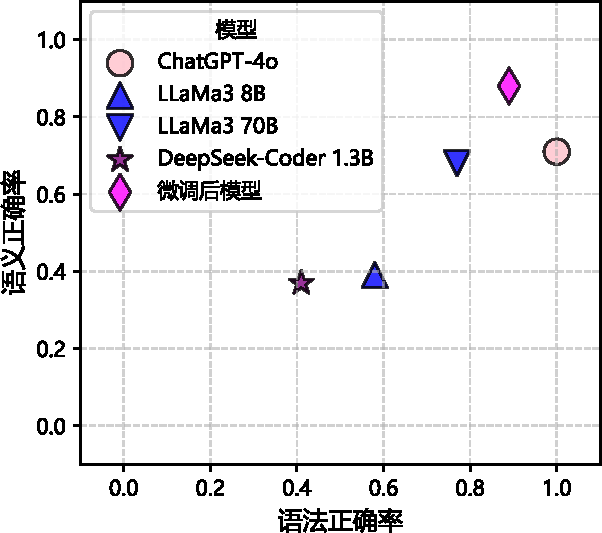
\includegraphics{figures/synatics_and_semantics-crop.pdf}
    \caption{各模型的语法正确率及语义正确率}
    \label{fig:syntactics_and_semantics}
\end{figure}
\begin{table}
    \centering
    \begin{tabular}{lcc}
        \toprule
        \textbf{模型} & \textbf{语法正确率} & \textbf{语义正确率} \\
        \midrule
        ChatGPT-4o & 1 & 0.71 \\
        LLaMA3 8B & 0.58 & 0.39 \\
        LLaMA3 70B & 0.77 & 0.68 \\
        DeepSeek-Coder 1.3B & 0.41 & 0.37 \\
        \midrule
        微调后模型 & 0.89 & 0.89 \\
        \bottomrule
    \end{tabular}
    \caption{各模型在语法和语义方面的对比分析}
    \label{fig:overall_syntactics_semantics}
\end{table}
\begin{table}[h]
    \centering
    \renewcommand{\arraystretch}{1.2}
    \setlength{\tabcolsep}{5pt}
    \resizebox{\textwidth}{!}{
    \begin{tabular}{lcccccccccccccccccc}
        \toprule
        \multirow{2}{*}{模型} & \multicolumn{2}{c}{猜测赋值} & \multicolumn{2}{c}{表达约束} & \multicolumn{2}{c}{生成组合} & \multicolumn{2}{c}{连接} & \multicolumn{2}{c}{传递闭包} & \multicolumn{2}{c}{表达偏好} & \multicolumn{2}{c}{按值过滤} & \multicolumn{2}{c}{负过滤}& \multicolumn{2}{c}{按数值比较过滤}  \\
        \cmidrule(lr){2-3} \cmidrule(lr){4-5} \cmidrule(lr){6-7} \cmidrule(lr){8-9} \cmidrule(lr){10-11} \cmidrule(lr){12-13} \cmidrule(lr){14-15} \cmidrule(lr){16-17} \cmidrule(lr){18-19}
        & \textit{语法} & \textit{语义} & \textit{语法} & \textit{语义} & \textit{语法} & \textit{语义} & \textit{语法} & \textit{语义} & \textit{语法} & \textit{语义} & \textit{语法} & \textit{语义} & \textit{语法} & \textit{语义} & \textit{语法} & \textit{语义} & \textit{语法} & \textit{语义}\\
        \midrule
        ChatGPT-4o & 1 & 0.8 & 1 & 1 & 1 & 1 & 1 & 1 & 1 & 1 & 1 & 0 & 1 & 0 & 1 & 0 & 1 & 1\\
        LLaMA3 8B & 0.6 & 0.4 & 0.5 & 0.5 & 0 & 0 & 0 & 0 & 1 & 0.7 & 0.3 & 0.3 & 0.4 & 0.4 & 0.2 & 0 & 0 & 0 \\
        LLaMA3 70B & 0.8 & 0.8 & 0.4 & 0.3 & 1 & 1 & 0.7 & 0.7 & 0.9 & 0.7 & 0 & 0 & 0.8 & 0.8 & 0.8 & 0.7 & 1 & 1\\
        DeepSeek-Coder 1.3B & 0.6 & 0.4 & 0.7 & 0.2 & 0 & 0 & 1 & 0.8 & 1 & 1 & 0 & 0 & 0.6 & 0.1 & 0.2 & 0 & 1 & 1 \\
        \midrule
        \textbf{微调后模型} & 1 & 0.9 & 1 & 1 & 0 & 0 & 1 & 1 & 1 & 1 & 1 & 1 & 1 & 1 & 0.8 & 0.7 & 1 & 1 \\
        \bottomrule
    \end{tabular}
    }
    \caption{不同模型在各ASP任务类型上的性能对比}
    \label{tab:semantics_comparison}
\end{table}

为了进一步检验模型的泛化能力(即面对未见过的自然语言描述时是否依然能正确生成 ASP 程序),本文额外生成了一个全新的拓展测试集。
实验对象仍选取上述实验中的所有模型。
拓展测试集仍保持与训练模板相似的基本任务类型(仍是九大类任务,如赋值、约束、组合等),但是表述风格更加丰富,包括
不同的描述方式、不同的关键词顺序、更多的冗余细节等等。
此外,引入了更多自然语言变化,以测试模型对语义理解的适应性。例如,在原本的训练集中的一种提示词为:“为每个 city(X) 元素选择一个标签,标签包括 moscow、rome、dubai。”
但是在拓展测试集中,改写为:“假设有城市集 city(X),请你从以下标签中为每个城市唯一地选一个:moscow,rome,dubai。”。
评估指标仍选取语法命中率和语义命中率。

具体实验结果见表\ref{tab:robust1}。
结果显示,经过微调后的DeepSeek-Coder 1.3B的语法正确率提高到了97\%,十分接近完全正确,这说明经过微调后的模型几乎不会产生语法错误。
语义正确率仍然保持在89\%,表明即使自然语言描述变化较大,模型依然能正确理解并生成对应 ASP 代码。

\begin{table}[h]
\centering
\begin{tabular}{lcc}
\toprule
\textbf{Model} & \textbf{Syntactic} & \textbf{Semantic} \\
\midrule
ChatGPT-4o     & 0.91   & 0.88 \\
DeepSeek-Coder 1.3B         & 0.60     & 0.57 \\
LLaMA3 8B      & 0.66     & 0.69 \\
LLaMA3 70B    & 0.89     & 0.85 \\
\midrule
\textbf{微调后模型}  & 0.97 & 0.89 \\
\bottomrule
\end{tabular}
\caption{拓展测试集上的结果}
\label{tab:robust1}
\end{table}
\subsection{规则修正与规则蒸馏实验}
规则修正与规则蒸馏实验的目的包括以下两方面:
\begin{enumerate}[nosep]
\item 验证添加视觉场景理解模块,支持多模态输入后的神经符号VQA框架对部分可见积木世界场景下空间推理问答的有效性。
\item 评估本文设计的ASP规则蒸馏方法对提升部分可见积木世界场景下空间推理问答准确率的效果。
\item 验证RCNSP在不同LLM上具有泛化能力。
\end{enumerate}

为了达到上述实验目的,本节实验对象选取目前主流的三种LLM:DeepSeek-Coder、LLaMA3和ChatGPT-4o。
以上既包含DeepSeek-Coder这类轻量级专用模型,
也涵盖ChatGPT-4o这类通用型先进系统,而LLaMA3性能和效率之间取得了平衡,属于居中水平的模型。
在多个基座上进行实验,可以有效证明RCNSP对不同LLM的泛化能力。
实验数据集选取本文第三章构建的POVQAD,将每条样本的图像、自然语言问题输入RCNSP,与每条样本的答案进行对比,计算
回答正确率。实验环境的配置方面,CPU为Intel Core i9 12900K,内存为128GB,显卡为2张Nvidia RTX4090。

基线模型一采用直接向 VLM 提问的方式,即将自然语言问题与图像一同输入 VLM,并不给予任何的额外提示。
直接提示VLM的方式虽然简单,却是评估模型的关键基准,因为直接提示方法能够反映模型在没有任何
外部推理辅助机制的情况下,自身对空间问题的处理能力。

基线模型二为原始框架方法,实际上相当于去除规则蒸馏模块的RCNSP。Wang等人设计的原始框架,是对StepGame、SparQA这种纯文本空间推理数据集
中的问题进行推理解答,不包括视觉场景理解,不支持多模态的输入。故去除规则蒸馏模块的RCNSP实际上相当于Wang等人设计的
框架的支持多模态输入的版本,使其能够顺利在第\ref{dataset}章设计的空间推理数据集上进行实验,
进而与本文添加规则蒸馏模块后的RCNSP框架形成对比。

实验结果见表\ref{tab:overall_comparison}。根据实验结果,RCNSP在三种LLM上均取得了较高的正确率,可以证明
RCNSP在不同的LLM上具有泛化能力。RCNSP相比原始框架方法,在DeepSeek-Coder 1.3B、LLaMA3 70B、ChatGPT-4o三种模型上的回答问题
正确率分别高出9.3\%、9.4\%、8.2\%,平均高出8.96\%,足以证明本文设计的规则蒸馏方法对提升部分可见积木世界场景下空间推理问答准确率
具有显著效果。原始框架方法在三种LLM的问答正确率均超过了直接提问方法,证明支持多模态输入后的神经符号VQA框架对部分可见积木世界场景下
的空间推理问答具有有效性。
\begin{table}[h]
    \centering
    \begin{tabular}{lc}
        \toprule
        \textbf{任务类型} & \textbf{正确率} \\
        \midrule
        \multicolumn{2}{c}{\textbf{DeepSeek-Coder 1.3B}} \\
        直接提问 & 59.4\% \\
        原始框架方法 & 72.5\% \\
        RCNSP & 81.8\% \\
        \midrule
        \multicolumn{2}{c}{\textbf{LLaMA3 70B}} \\
        直接提问 & 65.7\% \\
        原始框架方法 & 70.2\% \\
        RCNSP & 79.6\% \\
        \midrule
        \multicolumn{2}{c}{\textbf{ChatGPT-4o}} \\
        直接提问 & 71.5\% \\
        原始框架方法 & 76.6\% \\
        RCNSP & 84.8\% \\
        \bottomrule
    \end{tabular}
    \caption{不同模型及方法在各问题类型上的表现}
    \label{tab:overall_comparison}
\end{table}
\section{本章小结}
本章围绕设计一个规则自动补全的神经符号VQA框架的目标,从设计方案、核心技术及实现与实现分析三方面进行展开。

首先,介绍了RCNSP设计方案。围绕RCNSP的整体设计思路展开,与现有的神经符号框架进行对比,介绍各个模块的功能作用,并重点突出了规则蒸馏中规则自动补充的原理。

其次,介绍了RCNSP核心技术及实现。针对RCNSP中视觉场景理解、语义解析、迭代反馈与规则修正、规则蒸馏、ASP推理、求解结果翻译
这六个核心模块进行了详细阐述。特别是对于语义解析、迭代反馈与规则修正和规则蒸馏这三个模块进行了重点描述。

最后,进行了实验分析。在第三小节中,本文对语义解析微调实验、规则修正与规则蒸馏实验,从实验目的、实验对象、实验方法、实验环境及实验结果
分析上进行了阐述。
最终语义解析微调实验的结果证明了语义解析模块中,经过微调后的LLM在生成ASP程序方面的语法命中率和语义命中率均有明显提升。
规则修正与规则蒸馏实验的结果证明
神经符号方法对部分可见积木世界场景下空间推理问答有效,本文设计的ASP规则蒸馏方法可以显著提升部分可见积木世界场景下空间推理问答准确率,
同时也验证了RCNSP在不同LLM上具有泛化能力。

本章的RCNSP为后续开发积木世界VQA系统奠定了坚实基础。